\documentclass[border=9,tikz]{standalone}
\begin{document}
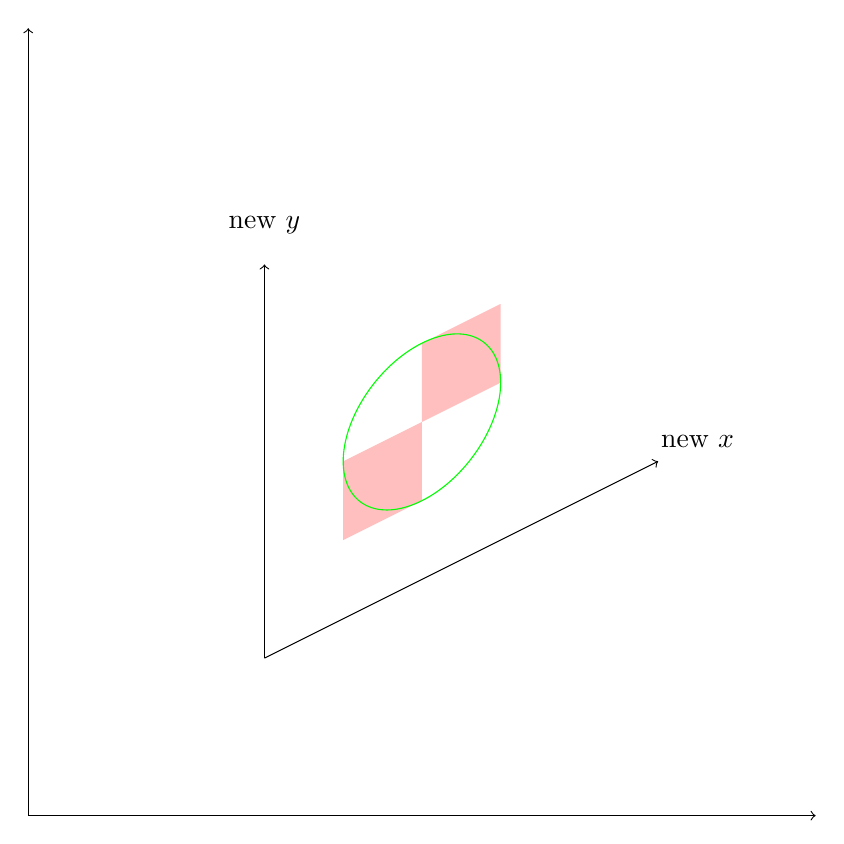
\begin{tikzpicture}
	\draw [->] (0, 0) -- (10, 0) ;
	\draw [->] (0, 0) -- (0, 10) ;
	
	\begin{scope} [ cm = {1, 0.5, 0, 1, (3, 2)}]
		\draw [->] (0, 0) -- (5, 0) node [pos = 1.1] {new $x$} ;
		\draw [->] (0, 0) -- (0, 5) node [pos = 1.1] {new $y$} ;
		\fill [pink] (1, 1) rectangle (2, 2) rectangle (3, 3);
		\draw [green] (2, 2) circle [radius = 1] ;
	\end{scope}
	
\end{tikzpicture}
\end{document}